

I thought it might be possible to identify each family by picking out the
constitutive member that had maximal or minimal dissipation and
production values; but for the numerical continuation of the gap solution
there doesn't seem to be any local maxima or minima. The benefit of this
type of analysis is that while there isn't any local maxima or minima for
the gap family, as I increase $L$ to its upper limits (in terms of being
able to converge the solution) the period of the solution grows extremely
quickly; in my mind making it more and more of an isolated solution. The
reason I hold this belief is that if we contemplate the family of gap
solutions in the context of the \KSe\ as a dynamical system, an
incredibly long period in this instance is actually prohibitive due to
the fact that the antisymmetric subspace $\bbU^+$ is a flow invariant
subspace. The idea I have is that the it is possible for \po 's to shadow
generic trajectories but as the period increases, it is essentially a
statement akin to ``the trajectory stays near the flow invariant subspace
for longer and longer periods of time" which (although I hesitate to use
this word) probabilistically doesn't seem likely.

In summary I suppose my thinking is that due to the fact that
antisymmetric \po 's lie in a flow invariant subspace $\bbU^+$ that
trajectories can neither leave nor enter then the period is a sort of
measure of how isolated these \po 's must be. In this regard I think that
the more relevant quantities would be a respective densities of scalar
quantities than the quantities themselves (average energy, dissipation,
etc.).

The numerical continuation of defect1 = \emph{rpo\_L13.2\_T15}  tile,
\reffig{fig:MNG_ppo_subdomains}\,(b), the first tile I entitled 'defect'
seems to be a member of the family of the reflection of the ``hook"
family: they are the same family up to discrete symmetry. My attempt
to demonstrate this is to take three representatives of each family in
\reffig{fig:MNG_leftright_family}, and show that at similar
spatiotemporal domains the solutions look very similar up to spatial and
temporal translations.
In this respect, one can see the family progresses from ``defect"
 to ``hook" to \reqv\, as $\tilde{L}$ increases.

My thought process on how to interpret this family goes as follows:
I don't know whether to interpret the ``hook" as a transition describing
breakdown of the \twot\ into a \reqv, or maybe as ``spatiotemporal
heteroclinic connection" but I am unsure if such a statement makes sense
in the absence of dynamics. Therefore I thought that maybe it makes sense
in terms of spatiotemporal symbolic dynamics. If one was playing sudoku
with spatiotemporal symbolic dynamics and there were symbols for defect
and \reqv, I think ``hook" would be a symbol that could fit in the
middle. Now, this doesn't really make sense because $\text{hook}\equiv
\text{defect}$ because they are members of the same family; it just gets
too complicated too quickly to extrapolate any ideas currently, much more
work required.

\begin{figure}
\begin{minipage}[height=.18\textheight]{.30\textwidth}
    \centering \small{\texttt{Defect1}}
    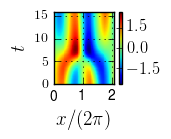
\includegraphics[width=\textwidth,height=.14\textheight]{MNG_rpo_L13d2_T15}
\end{minipage}%
\begin{minipage}[height=.18\textheight]{.30\textwidth}
\centering \small{\texttt{(a)}}
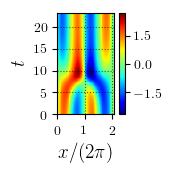
\includegraphics[width=\textwidth,height=.20\textheight]{MNG_rpo_L12p996_T23}
\end{minipage}%
\begin{minipage}[height=.18\textheight]{.30\textwidth}
\centering \small{\texttt{(b)}}
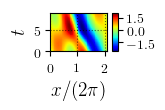
\includegraphics[width=\textwidth,height=.13\textheight]{MNG_rpo_L13p096_T8}
\end{minipage}%
\begin{minipage}[height=.18\textheight]{.30\textwidth}
\centering \small{\texttt{(c)}}
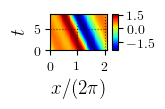
\includegraphics[width=\textwidth,height=.13\textheight]{MNG_reqv_L13p106_T8}
\end{minipage}
\\
\begin{minipage}[height=.18\textheight]{.30\textwidth}
    \centering \small{\texttt{hook}}
    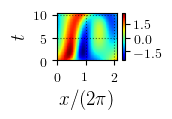
\includegraphics[width=\textwidth,height=.13\textheight]{MNG_rpo_L13p07_T10}
\end{minipage}%
\begin{minipage}[height=.18\textheight]{.30\textwidth}
    \centering \small{\texttt{(d)}}
    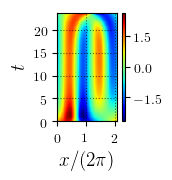
\includegraphics[width=\textwidth,height=.20\textheight]{MNG_rpo_L12p995_T23}
\end{minipage}%
\begin{minipage}[height=.18\textheight]{.30\textwidth}
    \centering \small{\texttt{(e)}}
    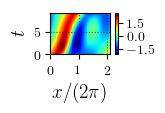
\includegraphics[width=\textwidth,height=.13\textheight]{MNG_rpo_L13p095_T9}
\end{minipage}%
\begin{minipage}[height=.18\textheight]{.30\textwidth}
    \centering \small{\texttt{(f)}}
    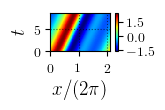
\includegraphics[width=\textwidth,height=.13\textheight]{MNG_reqv_L13p105_T8}
\end{minipage}
\caption{ \label{fig:MNG_leftright_family}
(a) \twoT\ \emph{rpo\_L12.996\_T23},
(b) \twot\ \emph{rpo\_L13.096\_T8},
(c) \reqv\ \emph{reqv\_L13.106\_T8}.
These three solutions were produced by numerical continuation in spatial
domain size of \twot\ defect1 = \emph{rpo\_L13.02\_T15}  tile
(see  \reffig{fig:MNG_ppo_subdomains}).
(d) \twoT\ \emph{rpo\_L12.995\_T23},
(e) \twot\ \emph{rpo\_L13.095\_T8},
(f) \reqv\ \emph{reqv\_L13.105\_T8}.
These three solutions were produced by numerical continuation in spatial
domain size of \twot\ hook = \emph{rpo\_L13.07\_T10} tile.
\twoTs\
(a) \emph{rpo\_L12.996\_T23} and
(d) \emph{rpo\_L12.995\_T23}
are the one and the same $\PO{(13.0,23)}\in\bbU^+$, differing only by
relative space and time shifts. The reflection symmetry is broken by the
nearby solution drifting either to the left or to the right, so (e,f)
belong to the right-drifting reflection of the left-drifting branch of
the solutions (a,b), \ie, they belong to the same branch of the
solution after the reduction of the spatial reflection symmetry.
In general, solutions can be distinguished or identified only after they
are sectioned and sliced, as done in \reffig{fig:MNG_hookequalsdefect}.
}
\end{figure}

\begin{figure}
\begin{minipage}[height=.32\textheight]{.8\textwidth}
\centering \small{\texttt{(a)}\qquad\qquad\texttt{(b)}}
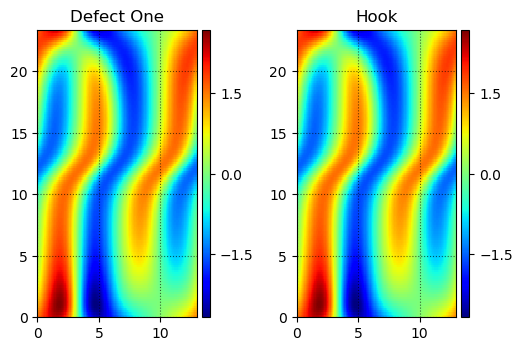
\includegraphics[width=\textwidth,height=.32\textheight]{MNG_hookequalsdefect}
\end{minipage}
\caption{ \label{fig:MNG_hookequalsdefect}
Continued from \reffig{fig:MNG_leftright_family}.
Sliced and sectioned minimal \twot\ solutions (not scaled relative to
others in repository; horizontal axis is $L$);
(a) Defect1 = \RPOtwot{13.2}{15} %\emph{rpo\_L13.2\_T15}
tile,
\reffig{fig:MNG_ppo_subdomains}\,(b), numerically continued to
$(\speriod{},\period{})=(12.996,23.373682)$.
(b) Reflection of the hook  = \RPOtwot{13.07}{10} %\emph{rpo\_L13.07\_T10}
tile numerically
continued to $(\speriod{},\period{}) = (12.996,23.373670)$.
}
\end{figure}

\begin{figure}
\begin{minipage}[height=.20\textheight]{.8\textwidth}
\centering \small{\texttt{(a)}}
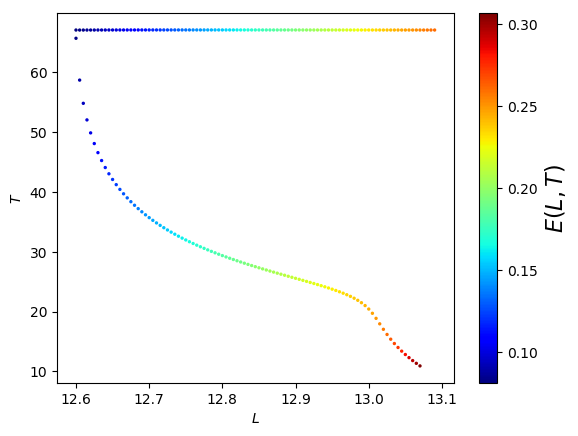
\includegraphics[width=\textwidth,height=.32\textheight]{MNG_hook_space_cont}
\end{minipage}
\caption{ \label{fig:MNG_hook_spatial_cont}
Bifurcation diagram plotted in $(\speriod{},\period{})$ plane.
Two branches resulting from numerical continuation in $L$ of
the hook  = \RPOtwot{13.07}{10} %\emph{rpo\_L13.07\_T10}
tiles family. $L$ was decreased until the
Gauss-Newton method failed; at which point, the numerical continuation
began increasing $L$ to test for hysteresis. This can be seen by the fact
that the bifucation diagram has two branches.
}
\end{figure}

\begin{figure}
\begin{minipage}[height=.20\textheight]{.8\textwidth}
\centering \small{\texttt{(a)}}
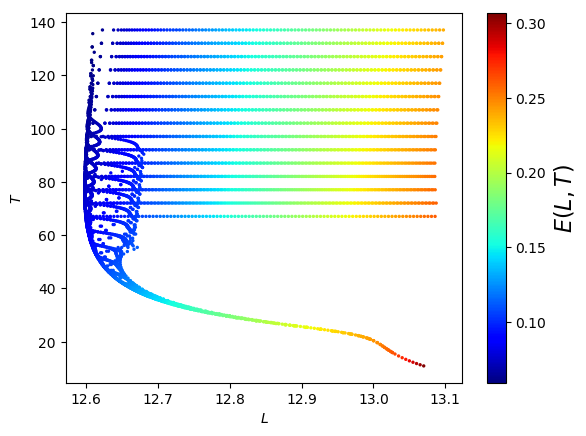
\includegraphics[width=\textwidth,height=.32\textheight]{MNG_st_cont}
\end{minipage}
\caption{ \label{fig:MNG_hook_st_cont}
Bifurcation diagram plotted in $(\speriod{},\period{})$ plane; numerical continuation of all points in \reffig{fig:MNG_hook_spatial_cont}.
These points were acquired by increasing $T$ and then decreasing $T$ via numerical continuation of both the lower and upper spatial continuation branches. The step size that $T$ was changed by was $\Delta T = 5$; smaller step sizes and smaller ranges seem to indicate that each branch is a one dimensional family.
}
\end{figure}

\begin{figure}
\begin{minipage}[height=.20\textheight]{.8\textwidth}
\centering \small{\texttt{(a)}}
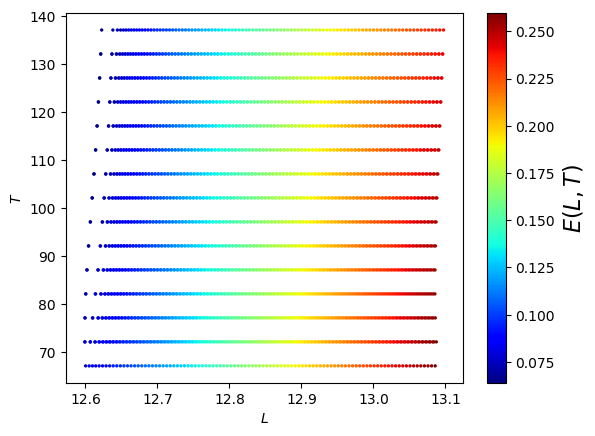
\includegraphics[width=\textwidth,height=.32\textheight]{MNG_upper_dT5}
\end{minipage}
\caption{ \label{fig:MNG_upper_dT5}
Bifurcation diagram plotted in $(\speriod{},\period{})$ plane; numerical continuation of upper branch of \reffig{fig:MNG_hook_spatial_cont}.
These points were acquired by increasing $T$ and then decreasing $T$ via numerical continuation of the upper spatial continuation branch. The step size that $T$ was changed by was $\Delta T = 5$; smaller step sizes and smaller ranges seem to indicate that each branch is a one dimensional family.
}
\end{figure}


\begin{figure}
\begin{minipage}[height=.20\textheight]{.30\textwidth}
\centering \small{\texttt{(a)}}
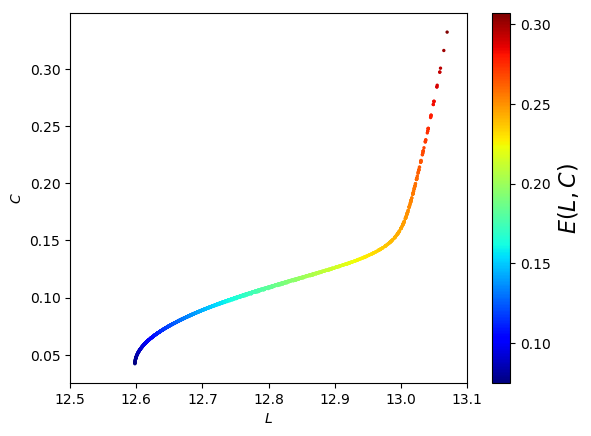
\includegraphics[width=\textwidth,height=.16\textheight]{MNG_LC_dT1}
\end{minipage}
\begin{minipage}[height=.20\textheight]{.30\textwidth}
\centering \small{\texttt{(b)}}
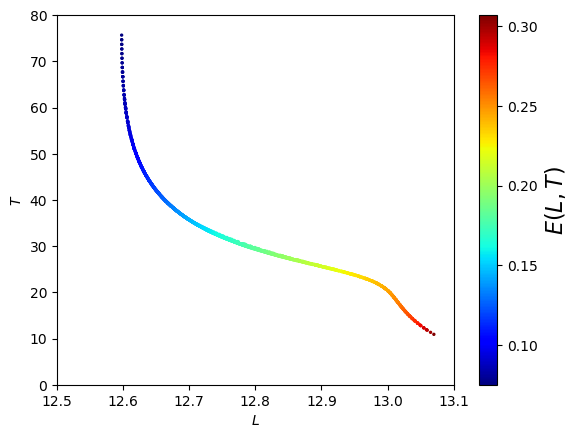
\includegraphics[width=\textwidth,height=.16\textheight]{MNG_LT_dT1}
\end{minipage}
\begin{minipage}[height=.20\textheight]{.30\textwidth}
\centering \small{\texttt{(c)}}
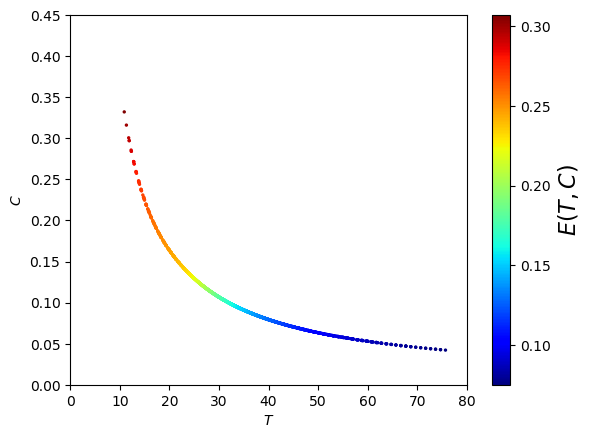
\includegraphics[width=\textwidth,height=.16\textheight]{MNG_TC_dT1}
\end{minipage}
\caption{ \label{fig:MNG_lower_dT1}
Numerical continuation of the lower spatial continuation branch of
\reffig{fig:MNG_hook_spatial_cont} by decreasing $T$ by 10 with step
sizes of $\Delta T = 1$. Plots in (a)$(L,C)$ plane (b) $(\speriod{},\period{})$ plane
(c) $(T,C)$ plane. Spatiotemporal energy is color coded.
}
\end{figure}

\begin{figure}
\begin{minipage}[height=.20\textheight]{.30\textwidth}
\centering \small{\texttt{(a)}}
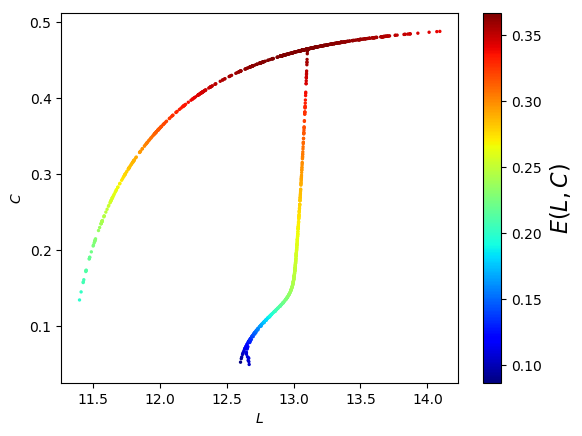
\includegraphics[width=\textwidth,height=.16\textheight]{MNG_LC_dT5}
\end{minipage}
\begin{minipage}[height=.20\textheight]{.30\textwidth}
\centering \small{\texttt{(b)}}
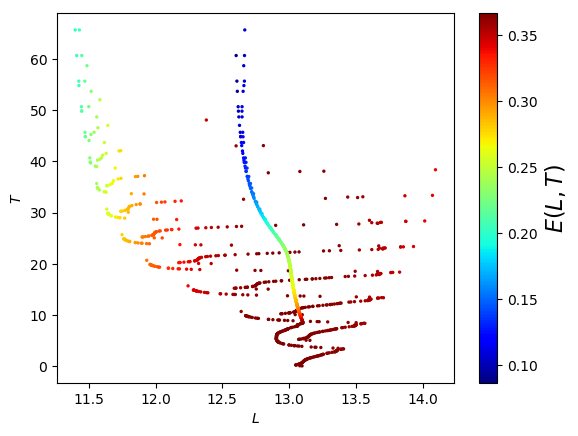
\includegraphics[width=\textwidth,height=.16\textheight]{MNG_LT_dT5}
\end{minipage}
\begin{minipage}[height=.20\textheight]{.30\textwidth}
\centering \small{\texttt{(c)}}
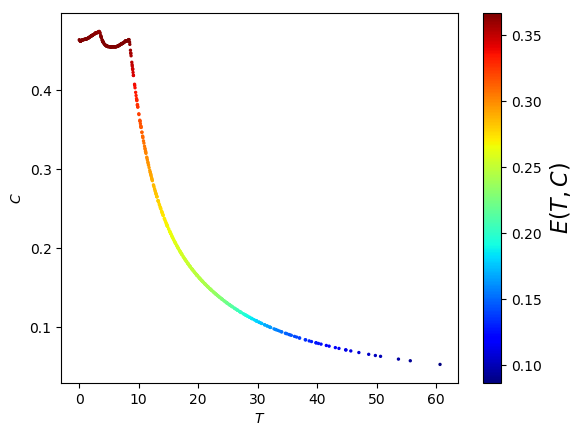
\includegraphics[width=\textwidth,height=.16\textheight]{MNG_TC_dT5}
\end{minipage}
\caption{ \label{fig:MNG_lower_dT5}
Numerical continuation of the lower spatial continuation branch of
\reffig{fig:MNG_hook_spatial_cont} by decreasing $T$ by as much as possible
(while still remaining positive) with step
sizes of $\Delta T = 5$. Plots in (a) $(L,C)$ plane, (b) $(\speriod{},\period{})$ plane, and
(c) $(T,C)$ plane. Spatiotemporal energy is color coded.
}
\end{figure}
